\chapter{User Interface}
\label{chap:user_interface}

\section{Overview}

\section{Menu and toolbar actions}
  
  \begin{description}
   \item[{
\includegraphics[width=0.5cm]{../../icons/document-open.png} File -> Open...}] 
   \item[{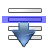
\includegraphics[width=0.5cm]{../../icons/listDown.png} File -> Next File}] 
   \item[{
\includegraphics[width=0.5cm]{../../icons/listUp.png} File -> Previous File}] 
   
   \item[{
\includegraphics[width=0.5cm]{../../icons/extractNormalization.png} Reduction -> Set Normalization}] 
   \item[{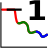
\includegraphics[width=0.5cm]{../../icons/totalReflection.png} Reduction -> Set Scaling}] 
   
   \item[{
\includegraphics[width=0.5cm]{../../icons/addRef.png} Reduction -> Keep Item in List}] 
   \item[{
\includegraphics[width=0.5cm]{../../icons/delRef.png} Reduction -> Remove Line}] 
   \item[{
\includegraphics[width=0.5cm]{../../icons/clearRef.png} Reduction -> Clear List}] 

    \item[{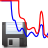
\includegraphics[width=0.5cm]{../../icons/reduce.png} Reduction -> Reduce...}] 

   \item[{
\includegraphics[width=0.5cm]{../../icons/findXauto.png} Advanced -> Automatic Peak Finder}] 
   \item[{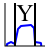
\includegraphics[width=0.5cm]{../../icons/limitYauto.png} Advanced -> Automatic Y Limits}] 
   \item[{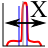
\includegraphics[width=0.5cm]{../../icons/fitXPos.png} Advanced -> Refine X}] 
   \item[{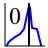
\includegraphics[width=0.5cm]{../../icons/tthZero.png} Advanced -> Adjust Direct Beam}] 
   \item[{ Advanced -> Clear Overwrite}] 
  \end{description}

\section{Docked Windows}
  Dock windows are the the regions on the left and right of the window containing e.g. the projection plots and extraction parameters. They are visible on any tab of the main interface.
  These windows positions can be customized by the user anywhere around the center, on top of each other, detached from the main window or completely closed (will be saved on exit). Closed dock windows can be restored by right clicking any dock window title or the empty region next to the toolbar and menu. You can easily detach and reattach them by clicking the diamod button at the top right.
  Here is a list of available dock windows:
  
  \begin{description}
   \item[Files] A list of all datafile in the current directory together with an entry to search for a file by number and select to extract either histogram or event mode data.
   \item[X-Projection] A plot with the data of the loaded file projected on the detector X-axis. Green lines indicate the background region defined at the moment. The X-position is marked with a black line and the X-width with two red lines. The mouse can be used to change the background region and X-center using the left mouse button and set the X-width using the right mouse button.
   \item[Y-Projection] An equivalent projection on the detector Y-axis, showing the selected Y-region with red lines. The mouse can be used to change the Y-region using left clicks.
   \item[Reflectivity] Show all datasets already added to the reduction list and the currently selected one. For unnormalized datasets it show intensity and background vs. wavelength. Datasets in the reduction list can be scaled with the mouse wheel when at the right x-coordinates (faster scaling when CTRL is pressed while scrolling).
   \item[Reflectivity Extraction] The parameters used to extract the active reflectivity. When adding a dataset to the reduction list, these parameters are stored.
   \item[Plot Options] Global settings for the shown plots, does not effect the data reduction in any way. Here you can also chose to show the 2D datasets in wavelength and angle instead of time of flight and pixel.
   \item[Advanced Background] Additional parameters for the background subtraction, normally not in use.
   \item[Advanced Parameters] Settings to change the extraction method or overwrite parameters otherwise read from the datafile.
   \item[Algorithm Parameters] Settings for the peak finder and curve stitching algorithms.
   \item[Event Mode Readout] Define the binning to be used when reading event mode data.
  \end{description}


\section{Plots}

\section{Data reduction table}

